% Options for packages loaded elsewhere
\PassOptionsToPackage{unicode}{hyperref}
\PassOptionsToPackage{hyphens}{url}
\PassOptionsToPackage{dvipsnames,svgnames,x11names}{xcolor}
%
\documentclass[
  letterpaper,
  DIV=11,
  numbers=noendperiod]{scrreport}

\usepackage{amsmath,amssymb}
\usepackage{iftex}
\ifPDFTeX
  \usepackage[T1]{fontenc}
  \usepackage[utf8]{inputenc}
  \usepackage{textcomp} % provide euro and other symbols
\else % if luatex or xetex
  \usepackage{unicode-math}
  \defaultfontfeatures{Scale=MatchLowercase}
  \defaultfontfeatures[\rmfamily]{Ligatures=TeX,Scale=1}
\fi
\usepackage{lmodern}
\ifPDFTeX\else  
    % xetex/luatex font selection
\fi
% Use upquote if available, for straight quotes in verbatim environments
\IfFileExists{upquote.sty}{\usepackage{upquote}}{}
\IfFileExists{microtype.sty}{% use microtype if available
  \usepackage[]{microtype}
  \UseMicrotypeSet[protrusion]{basicmath} % disable protrusion for tt fonts
}{}
\makeatletter
\@ifundefined{KOMAClassName}{% if non-KOMA class
  \IfFileExists{parskip.sty}{%
    \usepackage{parskip}
  }{% else
    \setlength{\parindent}{0pt}
    \setlength{\parskip}{6pt plus 2pt minus 1pt}}
}{% if KOMA class
  \KOMAoptions{parskip=half}}
\makeatother
\usepackage{xcolor}
\setlength{\emergencystretch}{3em} % prevent overfull lines
\setcounter{secnumdepth}{5}
% Make \paragraph and \subparagraph free-standing
\ifx\paragraph\undefined\else
  \let\oldparagraph\paragraph
  \renewcommand{\paragraph}[1]{\oldparagraph{#1}\mbox{}}
\fi
\ifx\subparagraph\undefined\else
  \let\oldsubparagraph\subparagraph
  \renewcommand{\subparagraph}[1]{\oldsubparagraph{#1}\mbox{}}
\fi


\providecommand{\tightlist}{%
  \setlength{\itemsep}{0pt}\setlength{\parskip}{0pt}}\usepackage{longtable,booktabs,array}
\usepackage{calc} % for calculating minipage widths
% Correct order of tables after \paragraph or \subparagraph
\usepackage{etoolbox}
\makeatletter
\patchcmd\longtable{\par}{\if@noskipsec\mbox{}\fi\par}{}{}
\makeatother
% Allow footnotes in longtable head/foot
\IfFileExists{footnotehyper.sty}{\usepackage{footnotehyper}}{\usepackage{footnote}}
\makesavenoteenv{longtable}
\usepackage{graphicx}
\makeatletter
\def\maxwidth{\ifdim\Gin@nat@width>\linewidth\linewidth\else\Gin@nat@width\fi}
\def\maxheight{\ifdim\Gin@nat@height>\textheight\textheight\else\Gin@nat@height\fi}
\makeatother
% Scale images if necessary, so that they will not overflow the page
% margins by default, and it is still possible to overwrite the defaults
% using explicit options in \includegraphics[width, height, ...]{}
\setkeys{Gin}{width=\maxwidth,height=\maxheight,keepaspectratio}
% Set default figure placement to htbp
\makeatletter
\def\fps@figure{htbp}
\makeatother

%%%% header.tex

%packages
\usepackage{mathtools}

%macros
\DeclareMathOperator{\vol}{vol}
\DeclareMathOperator{\U}{U}
\DeclareMathOperator{\SU}{SU}
\DeclareMathOperator{\imunit}{i}
\DeclareMathOperator{\id}{id}
\newcommand{\stdim}{D}


%%%% end header.tex
\KOMAoption{captions}{tableheading}
\makeatletter
\@ifpackageloaded{tcolorbox}{}{\usepackage[skins,breakable]{tcolorbox}}
\@ifpackageloaded{fontawesome5}{}{\usepackage{fontawesome5}}
\definecolor{quarto-callout-color}{HTML}{909090}
\definecolor{quarto-callout-note-color}{HTML}{0758E5}
\definecolor{quarto-callout-important-color}{HTML}{CC1914}
\definecolor{quarto-callout-warning-color}{HTML}{EB9113}
\definecolor{quarto-callout-tip-color}{HTML}{00A047}
\definecolor{quarto-callout-caution-color}{HTML}{FC5300}
\definecolor{quarto-callout-color-frame}{HTML}{acacac}
\definecolor{quarto-callout-note-color-frame}{HTML}{4582ec}
\definecolor{quarto-callout-important-color-frame}{HTML}{d9534f}
\definecolor{quarto-callout-warning-color-frame}{HTML}{f0ad4e}
\definecolor{quarto-callout-tip-color-frame}{HTML}{02b875}
\definecolor{quarto-callout-caution-color-frame}{HTML}{fd7e14}
\makeatother
\makeatletter
\makeatother
\makeatletter
\@ifpackageloaded{bookmark}{}{\usepackage{bookmark}}
\makeatother
\makeatletter
\@ifpackageloaded{caption}{}{\usepackage{caption}}
\AtBeginDocument{%
\ifdefined\contentsname
  \renewcommand*\contentsname{Table of contents}
\else
  \newcommand\contentsname{Table of contents}
\fi
\ifdefined\listfigurename
  \renewcommand*\listfigurename{List of Figures}
\else
  \newcommand\listfigurename{List of Figures}
\fi
\ifdefined\listtablename
  \renewcommand*\listtablename{List of Tables}
\else
  \newcommand\listtablename{List of Tables}
\fi
\ifdefined\figurename
  \renewcommand*\figurename{Figure}
\else
  \newcommand\figurename{Figure}
\fi
\ifdefined\tablename
  \renewcommand*\tablename{Table}
\else
  \newcommand\tablename{Table}
\fi
}
\@ifpackageloaded{float}{}{\usepackage{float}}
\floatstyle{ruled}
\@ifundefined{c@chapter}{\newfloat{codelisting}{h}{lop}}{\newfloat{codelisting}{h}{lop}[chapter]}
\floatname{codelisting}{Listing}
\newcommand*\listoflistings{\listof{codelisting}{List of Listings}}
\makeatother
\makeatletter
\@ifpackageloaded{caption}{}{\usepackage{caption}}
\@ifpackageloaded{subcaption}{}{\usepackage{subcaption}}
\makeatother
\makeatletter
\@ifpackageloaded{tcolorbox}{}{\usepackage[skins,breakable]{tcolorbox}}
\makeatother
\makeatletter
\@ifundefined{shadecolor}{\definecolor{shadecolor}{rgb}{.97, .97, .97}}
\makeatother
\makeatletter
\makeatother
\makeatletter
\makeatother
\ifLuaTeX
  \usepackage{selnolig}  % disable illegal ligatures
\fi
\usepackage[style=phys,eprint=true,url=true,backref=true,biblabel=brackets,citestyle
= numeric-comp,sorting = none]{biblatex}
\addbibresource{references.bib}
\IfFileExists{bookmark.sty}{\usepackage{bookmark}}{\usepackage{hyperref}}
\IfFileExists{xurl.sty}{\usepackage{xurl}}{} % add URL line breaks if available
\urlstyle{same} % disable monospaced font for URLs
\hypersetup{
  pdftitle={A Lecture on Topological Operators},
  pdfauthor={Kantaro Ohmori},
  colorlinks=true,
  linkcolor={blue},
  filecolor={Maroon},
  citecolor={Blue},
  urlcolor={Blue},
  pdfcreator={LaTeX via pandoc}}

\title{A Lecture on Topological Operators}
\author{Kantaro Ohmori}
\date{2023-11-25}

\begin{document}
\maketitle
\ifdefined\Shaded\renewenvironment{Shaded}{\begin{tcolorbox}[boxrule=0pt, enhanced, frame hidden, borderline west={3pt}{0pt}{shadecolor}, breakable, interior hidden, sharp corners]}{\end{tcolorbox}}\fi

\renewcommand*\contentsname{Table of contents}
{
\hypersetup{linkcolor=}
\setcounter{tocdepth}{2}
\tableofcontents
}
\bookmarksetup{startatroot}

\hypertarget{what-is-this}{%
\chapter*{What is this}\label{what-is-this}}
\addcontentsline{toc}{chapter}{What is this}

\markboth{What is this}{What is this}

\(\vol\) This is a lecture note prepared for two sets of ``intensive
lectures'':\footnote{In Japan, an ``intensive lecture'' is a format of a
  lecture course where a lecturer (usually from another university)
  gives lectures in consecutive days filling 7-9 slots in usually 3
  days.}

\begin{itemize}
\tightlist
\item
  at Tohoku University, Oct.~11-13, 2023, and
\item
  at Yukawa Insititute for Theoretical Physics, Kyoto University,
  Nov.~29-1, 2023.
\end{itemize}

In this lecture I will try to explain the constructions of topological
defects corresponding to generalized symmetries. Due to lack of time and
(more significantly) my understanding, the lecture will focus on bosonic
systems, and the generalization to fermionic systems is left for the
readers/audiences.

\begin{tcolorbox}[enhanced jigsaw, colbacktitle=quarto-callout-warning-color!10!white, opacitybacktitle=0.6, bottomrule=.15mm, titlerule=0mm, colframe=quarto-callout-warning-color-frame, colback=white, leftrule=.75mm, toprule=.15mm, bottomtitle=1mm, opacityback=0, title=\textcolor{quarto-callout-warning-color}{\faExclamationTriangle}\hspace{0.5em}{Warning}, toptitle=1mm, arc=.35mm, coltitle=black, breakable, left=2mm, rightrule=.15mm]

This note is \textbf{under construction}, and there are many missed
equations, figures, explanations, sections, and \emph{references}.

\end{tcolorbox}

\hypertarget{prerequisite}{%
\section*{Prerequisite}\label{prerequisite}}
\addcontentsline{toc}{section}{Prerequisite}

\markright{Prerequisite}

\begin{itemize}
\tightlist
\item
  Basic knowledge about scalar field theory and (abelian) gauge theory
  in path-integral formalism, and
\item
  Knowledge about renormalization group (RG) flows to understand
  motivations.
\item
  Knowledge about differential form and Stokes's theorem in terms of it.
\end{itemize}

\hypertarget{what-is-contained-and-what-is-not}{%
\section*{What is contained and what is
not}\label{what-is-contained-and-what-is-not}}
\addcontentsline{toc}{section}{What is contained and what is not}

\markright{What is contained and what is not}

\hypertarget{other-lecturesreviews}{%
\section*{Other Lectures/Reviews}\label{other-lecturesreviews}}
\addcontentsline{toc}{section}{Other Lectures/Reviews}

\markright{Other Lectures/Reviews}

Recently there has been a surge of lecture notes/ review articles on
generalized symmetries. The ones I have noticed are
\autocite{McGreevy:2022oyu,Schafer-Nameki:2023jdn,Gomes:2023ahz,Bhardwaj:2023kri,Luo:2023ive,Shao:2023gho}.
Because this lecture will focus on the fundamental aspects of the topic
and will not connect very well with the existent literature (so sorry
about that), readers/audiences are strongly encouraged to refer to at
least one of them, or something similar.

Also, about conventional symmetries and their anomalies, there are nice
old lectures. The one I would particularly recommend is
\autocite{TachikawaTasi}.

\bookmarksetup{startatroot}

\hypertarget{introduction}{%
\chapter{Introduction}\label{introduction}}

\hypertarget{symmetry}{%
\section{Symmetry}\label{symmetry}}

\textbf{Symmetry} plays a fundamental role in theoretical physics. In
this lecture we consider them in \emph{quantum field theories} (QFTs).
The fundamental fact about symmetry in QFTs is that is it preserved
along the renormalization group flow. More precisely, when an
ultraviolet (UV) theory \(\mathcal{T}_\text{UV}\) flows into an infrared
theory \(\mathcal{T}_\text{IR}\), there is a canonical homomorphism
\(f_\text{RG}\) from the UV symmetry group \(G_\text{UV}\) to the IR
symmetry group \(G_\text{IR}\):\footnote{If the UV theory is a fixed
  point, \(G_\text{UV}\) should be understood as the one preserved by
  the perturbation triggering the RG flow. If the RG flow is to a lower
  nonzero energy, and if one retains all the (even very massive) degrees
  of freedom in the description of \(\mathcal{T}_\text{IR}\), the map
  \(f_\text{RG}\) is an isomorphism. However, typically one integrates
  out massive dofs in the description of \(\mathcal{T}_\text{RG}\), in
  which case some symmetry can decouple and thus \(f_\text{RG}\) can be
  non-surjective. Also, if one also drops some higher-order interaction
  terms, or runs the flow to the zero energy, there can be an
  \emph{emergent} symmetry, in which case \(f_\text{RG}\) can be
  non-injective.}

\begin{tcolorbox}[enhanced jigsaw, colbacktitle=quarto-callout-important-color!10!white, opacitybacktitle=0.6, bottomrule=.15mm, titlerule=0mm, colframe=quarto-callout-important-color-frame, colback=white, leftrule=.75mm, toprule=.15mm, bottomtitle=1mm, opacityback=0, title=\textcolor{quarto-callout-important-color}{\faExclamation}\hspace{0.5em}{\textsf{RG flow homomorphism from UV symmetry to IR symmetry}}, toptitle=1mm, arc=.35mm, coltitle=black, breakable, left=2mm, rightrule=.15mm]

\begin{equation}\protect\hypertarget{eq-RG-group-match}{}{
f_\text{RG} : G_\text{UV} \to G_\text{IR}.
}\label{eq-RG-group-match}\end{equation}

\end{tcolorbox}

Given this relation, there are two ways of applying symmetry in QFT:

\begin{itemize}
\tightlist
\item
  UV to IR: Given a microscopic model (e.g.~a model of elementary
  particles or electrons in a matter), constrain/guess what happens in
  the macroscopic scale.
\item
  IR to UV: Given some macroscopic phenomena, constrain/guess what could
  be the microscopic origin of it (e.g.~guessing QCD Lagrangian from
  hadron spectrum).
\end{itemize}

\begin{tcolorbox}[enhanced jigsaw, colbacktitle=quarto-callout-note-color!10!white, opacitybacktitle=0.6, bottomrule=.15mm, titlerule=0mm, colframe=quarto-callout-note-color-frame, colback=white, leftrule=.75mm, toprule=.15mm, bottomtitle=1mm, opacityback=0, title=\textcolor{quarto-callout-note-color}{\faInfo}\hspace{0.5em}{\textsf{Terminology (global symmetry)}}, toptitle=1mm, arc=.35mm, coltitle=black, breakable, left=2mm, rightrule=.15mm]

In this lecture, ``symmetry'' means a \emph{global} symmetry. Here
\emph{global} means that the symmetry operation acts on the entire
space. In addition, in most contents we exclude symmetries acting on the
spacetime out of consideration for simplicity.

\end{tcolorbox}

\hypertarget{locality}{%
\section{Locality}\label{locality}}

The second important keyword in this lecture is \textbf{locality}. By
the word quantum field theory, in most cases we implicitly mean
\emph{local} quantum field theory. This can roughly be explained by that
the action is written as the integration of Lagrangian density, which is
a local functional of fields over the spacetime.

Locality of QFT has a consequence with respect to symmetry: that is, in
most situations we only consider symmetries that \emph{preserves
locality}. In terms of fields, this means that the symmetry
transformation is local:

\begin{equation}\protect\hypertarget{eq-field-transform}{}{
\phi(x) \mapsto F(\phi(x)),
}\label{eq-field-transform}\end{equation} where \(F(\phi(x))\) is a
function depends on the \emph{local} value a field (or a collection of
fields and its derivatives) at the point \(x\). If the symmetry involves
a spacetime transformation, the point \(x\) in the right-hand side
should be replaced by the image of \(x\) under the symmetry. This
preservation of locality of a symmetry is the reason for the symmetry
relation in Equation~\ref{eq-RG-group-match}. This will be made clear in
the lecture.

However, not all the (locality-preserving) symmetry in QFT takes the
form of Equation~\ref{eq-field-transform}, which is called
\emph{classical symmetry}. There are types of symmetry called
\emph{topological symmetry} or \emph{quantum symmetry}, which arises
from topologically-nontrivial field configuration. Examples are the
winding symmetry in 1+1d compact boson, and the monopole symmetries in
2+1d abelian gauge theories. In many occurrences a topological/quantum
symmetry is mapped to a symmetry of type of
Equation~\ref{eq-field-transform} under a duality, and thus it should
also be considered as being locality-preserving.

From the modern perspective, the universal characterization of
locality-preserving symmetries is its correspondence to
\textbf{topological operators}. A topological operator
\(\mathcal{D}[W_n]\) in a QFT is an extended operator defined on a
\(n\)-dimensional submanifold of the spacetime and the correlators
containing it should be invariant under the smooth deformation of the
supporting manifold \(W_n\) (See Figure~\ref{fig-TopOpsDeform}).

\begin{figure}[t]

{\centering 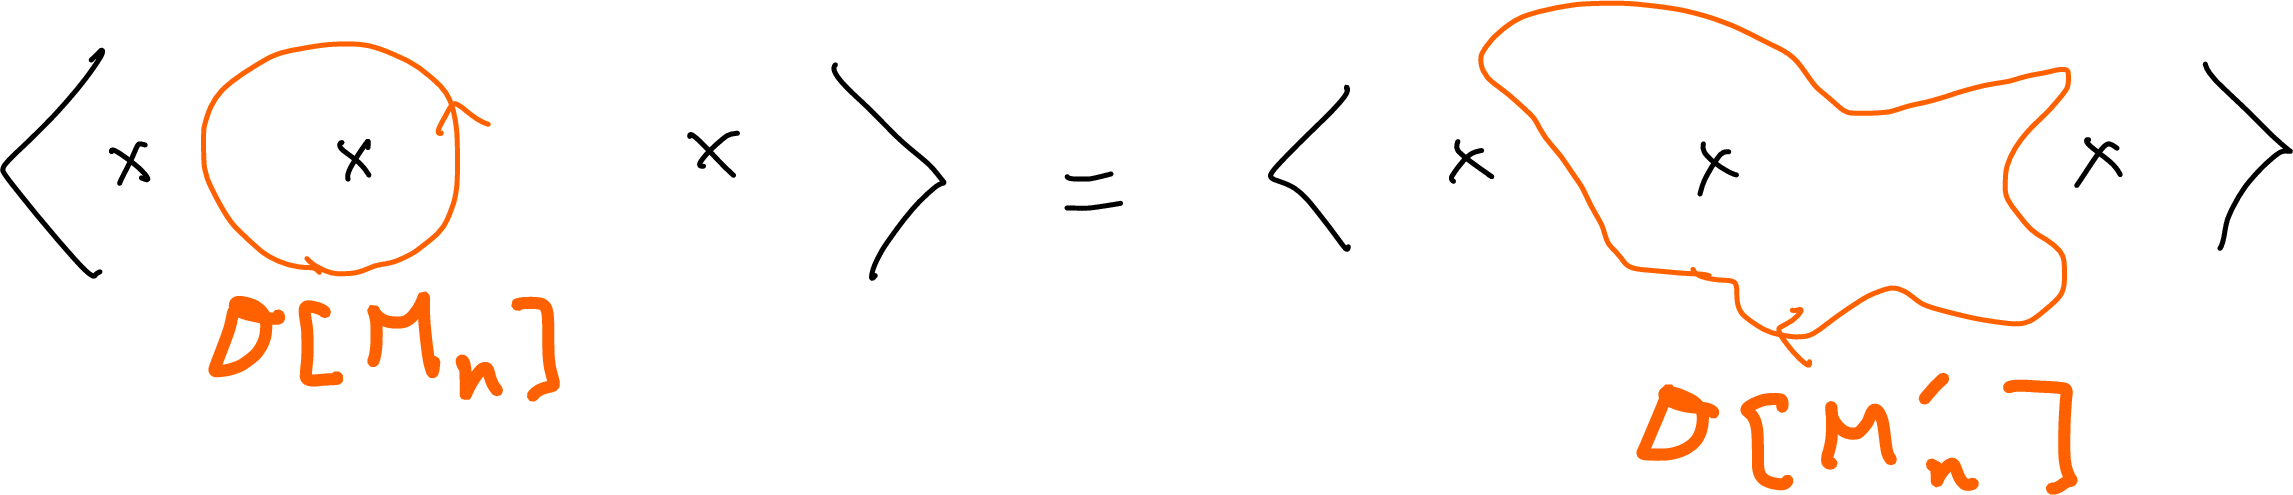
\includegraphics[width=4.16667in,height=\textheight]{figures/TopOpsDeform.png}

}

\caption{\label{fig-TopOpsDeform}Topological operator.}

\end{figure}

The first aim of the lecture is to understand the correspondence, that
is

\begin{tcolorbox}[enhanced jigsaw, colbacktitle=quarto-callout-important-color!10!white, opacitybacktitle=0.6, bottomrule=.15mm, titlerule=0mm, colframe=quarto-callout-important-color-frame, colback=white, leftrule=.75mm, toprule=.15mm, bottomtitle=1mm, opacityback=0, title=\textcolor{quarto-callout-important-color}{\faExclamation}\hspace{0.5em}{\textsf{Symmetry/Topological Operator Correspondence}}, toptitle=1mm, arc=.35mm, coltitle=black, breakable, left=2mm, rightrule=.15mm]

\begin{equation}\protect\hypertarget{eq-conv-STO-corresp}{}{\begin{split}
&\text{(Conventional) locality-preserving symmetry} \\ 
&\Longleftrightarrow\;
\text{invertible topological operator of codimension 1.}
\end{split}
}\label{eq-conv-STO-corresp}\end{equation}

\end{tcolorbox}

In this correspondence, the topological operator shoould be regarded as
the generalization of the \textbf{Noether charge} into possibly discrete
symmetry. To be precise, we regard this correspondence as the right-hand
side \emph{defining} the left-hand side. We will explicitly check this
correspondence/definition reproduces the known symmetries in the case of
a classical symmetry in a scalar field theory in
Chapter~\ref{sec-scalar}, and in the case of abelian gauge theory in
Chapter~\ref{sec-vector}. The case of fermion is very interesting and
crucial, but it will be remained to be worked out by audiences/readers.

\begin{tcolorbox}[enhanced jigsaw, colbacktitle=quarto-callout-note-color!10!white, opacitybacktitle=0.6, bottomrule=.15mm, titlerule=0mm, colframe=quarto-callout-note-color-frame, colback=white, leftrule=.75mm, toprule=.15mm, bottomtitle=1mm, opacityback=0, title=\textcolor{quarto-callout-note-color}{\faInfo}\hspace{0.5em}{\textsf{Terminology (locality-preserving)}}, toptitle=1mm, arc=.35mm, coltitle=black, breakable, left=2mm, rightrule=.15mm]

Again, we are \emph{not} talking about gauge redundancy, which is
sometimes called local symmetry. Global symmetries one encounters in a
QFT textbook are all locality-preserving.

\end{tcolorbox}

\begin{tcolorbox}[enhanced jigsaw, colbacktitle=quarto-callout-note-color!10!white, opacitybacktitle=0.6, bottomrule=.15mm, titlerule=0mm, colframe=quarto-callout-note-color-frame, colback=white, leftrule=.75mm, toprule=.15mm, bottomtitle=1mm, opacityback=0, title=\textcolor{quarto-callout-note-color}{\faInfo}\hspace{0.5em}{\textsf{Terminology (topological defect)}}, toptitle=1mm, arc=.35mm, coltitle=black, breakable, left=2mm, rightrule=.15mm]

Here is another unfortunate conflict of terminology. In the literature
(outside generalized symmetry literature), a ``topological defect''
refers to a dynamical object, or its trajectory viewed as an operator in
the IR theory, charg\textbf{ed} under a topological (higher) symmetry.
As an operator in the IR theory, it is \emph{not} a priori guaranteed to
be topological in the sense of Figure~\ref{fig-TopOpsDeform} . On the
other hand, in the generalized symmetry literature, ``topological defect
(operator)'' often means an extended operator that is itself
topological. In this lecture, in order to ease the confusion, we use the
term ``topological operator''.

\end{tcolorbox}

\hypertarget{generalized-symmetry}{%
\section{Generalized Symmetry}\label{generalized-symmetry}}

The correspondence in Equation~\ref{eq-conv-STO-corresp} is the core in
the notion of \textbf{generalized (global) symmetry}, coined by
\autocite{Gaiotto:2014kfa} \footnote{The global higher-form symmetry
  itself had appeared and investigated in the literature,
  e.g.~\autocite{Kapustin:2013uxa,Barkeshli:2014cna}, and its gauged
  version was essentially known from \autocite{KalbRamond}.}. That is,
the notion of symmetry can be generalized by relaxing the adjective in
the right-hand side of Equation~\ref{eq-conv-STO-corresp}. Therefore, we
\emph{define} generalized symmetry by the following correspondence
generalizing Equation~\ref{eq-conv-STO-corresp}:

\begin{tcolorbox}[enhanced jigsaw, colbacktitle=quarto-callout-important-color!10!white, opacitybacktitle=0.6, bottomrule=.15mm, titlerule=0mm, colframe=quarto-callout-important-color-frame, colback=white, leftrule=.75mm, toprule=.15mm, bottomtitle=1mm, opacityback=0, title=\textcolor{quarto-callout-important-color}{\faExclamation}\hspace{0.5em}{\textsf{Generalized Symmetry/Topological Operator Correspondence}}, toptitle=1mm, arc=.35mm, coltitle=black, breakable, left=2mm, rightrule=.15mm]

\begin{equation}\protect\hypertarget{eq-GSTO-corresp}{}{\begin{split}
&\text{Generalized symmetry (in a ``usual" QFT)} \\ 
&\stackrel{\text{def}}{\Longleftrightarrow}\;
\text{General topological operator.}
\end{split}
}\label{eq-GSTO-corresp}\end{equation}

\end{tcolorbox}

More specifically, a generalized symmetry corresponding to an operator
of codimension \(p+1\) is called \textbf{\(p\)-form symmetry}, and a
generalized symmetry corresponding to an operator without its inverse is
called \textbf{non-invertible symmetry} (among other names like category
symmetry and topological symmetry).

In an ``unusual'' QFT, we can even relax the topological-ness of the
operator in the right-hand side of Equation~\ref{eq-GSTO-corresp},
resulting in what is called \textbf{subsystem} symmetry. We will briefly
make a comment on it in Section~\ref{sec-trivial-scalar}.

The subclasses of generalized symmetry is summarized in the table below:

\hypertarget{tbl-sym-classes}{}
\begin{longtable}[]{@{}llll@{}}
\caption{\label{tbl-sym-classes}Subclasses of generalized symmetry and
defining properties of their corresponding topological
operators.}\tabularnewline
\toprule\noalign{}
& \(p\)-form & non-invertible & subsystem \\
\midrule\noalign{}
\endfirsthead
\toprule\noalign{}
& \(p\)-form & non-invertible & subsystem \\
\midrule\noalign{}
\endhead
\bottomrule\noalign{}
\endlastfoot
codimension & \(p+1\) & & \\
Invertible? & & No & \\
Topological? & & & Partically \\
\end{longtable}

The subclasses are not mutually exclusive, so, in principle, there can
be a 2-form non-invertible subsystem symmetry.

\hypertarget{contents-of-the-lecture}{%
\section{Contents of the Lecture}\label{contents-of-the-lecture}}

\textbf{FIXME}

\bookmarksetup{startatroot}

\hypertarget{sec-scalar}{%
\chapter{Topological Operators for Classical
Symmetry}\label{sec-scalar}}

In this section we take the classical symmetry in scalar field theory as
an example to study topological operators.

\hypertarget{set-up}{%
\section{Set Up}\label{set-up}}

To be concrete, let us consider the complex scalar field theory whose
Lagrangian (density) on a spacetime of dimension \(\stdim\) is given by
\[
\begin{aligned}
\mathcal{L}(\phi) &=  - \left(\frac12 \partial_\mu \phi(x)^* \partial^\nu \phi(x) + V(\phi(x))\right)\vol\\
&= \frac{1}{2} \mathop{d\phi} \wedge *\mathop{d\phi} - V(\phi(x))\vol,
\end{aligned}
\] where \(\mathop{*}\) is the Hodge star,
\(\vol = \mathop{*} 1 = \prod_{i=1}^{\stdim} \mathop{dx_i}\) is the
volume form for the flat space, and \(V(\phi)\) is the potential. The
action is the integral over the spacetime \(M\) (without boundary): \[
S[\phi] = \int_{M}\mathcal{L}(\phi).
\]

We consider a symmetry transformation of the scalar field
\begin{equation}\protect\hypertarget{eq-scalar-transf}{}{
\phi(x) \mapsto \phi^g(x)
}\label{eq-scalar-transf}\end{equation} parametrized by a group element
\(g\) (constant over \(M\)) that leaves the action invariant:
\begin{equation}\protect\hypertarget{eq-action-inv}{}{
S[\phi]=S[\phi^g].
}\label{eq-action-inv}\end{equation} This means that the Lagrangian is
invariant up to a total derivative:
\begin{equation}\protect\hypertarget{eq-Lagrangian-inv}{}{
\mathcal{L}(\phi^g) = \mathcal{L}(\phi) + \mathop{ds}(\phi,g) 
}\label{eq-Lagrangian-inv}\end{equation} where \(s(\phi,g)\) is a
\((\stdim-1)\)-form on \(M\) depending on the constant \(g\) and the
field \(\phi\). We set \(s(\phi,g=\id) = 0\), where \(\id\) is the unit
of the symmetry group. Then, by \(\phi = (\phi^g)^{g^{-1}}\), we can set
that \(s(\phi,g) = - s(\phi,g^{-1})\).

For example, the usual \(\U(1)\) rotation corresponds to the
transformation \[
\phi^g(x) = \mathop{g} \phi(x),
\] where \(g=e^{\imunit \alpha}\) is a \(\U(1)\) phase. The potential
\(V(\phi)\) might partially break the \(\U(1)\) rotation into its
subgroup \(\mathbb{Z}_k\), e.g.~\(V(\phi)\propto \phi^k+(\phi^*)^k\). In
such a case the parameter \(g\) takes \emph{discrete} values:
\(g = e^{\imunit \frac{2\pi i}{k}}\), \(i= 0 \cdots k-1\).

In addition, when \(V(\phi)=0\), the action \(S[\phi]\) also admit the
shift symmetry\footnote{If we use the form of Lagrangian
  \(\mathcal{L}^\prime= -\frac12 \phi \mathop{d*d\phi}\), this also
  gives an example where the total derivative in
  Equation~\ref{eq-Lagrangian-inv} is nonzero:
  \(s=-\frac12 \alpha \mathop{*}\mathop{d\phi}\).} \[
\phi^{\alpha}(x) = \phi(x) + \alpha.
\]

In this section, we would like to construct the \textbf{topological
operator} corresponding to these \emph{classical} symmetry.

\begin{tcolorbox}[enhanced jigsaw, colbacktitle=quarto-callout-note-color!10!white, opacitybacktitle=0.6, bottomrule=.15mm, titlerule=0mm, colframe=quarto-callout-note-color-frame, colback=white, leftrule=.75mm, toprule=.15mm, bottomtitle=1mm, opacityback=0, title=\textcolor{quarto-callout-note-color}{\faInfo}\hspace{0.5em}{\textsf{Note}}, toptitle=1mm, arc=.35mm, coltitle=black, breakable, left=2mm, rightrule=.15mm]

The construction will apply to other types of scalar field theory,
e.g.~real and/or multiple scalar fieldsas long as the kinetic term is
standard enough (more on this in Section~\ref{sec-trivial-scalar}). For
non-linear sigma model with topologically non-trivial target, the
Lagrange multiplier \(\lambda\) below should take values in the correct
set. We will consider the case with \(S^1\) target (compact boson) in
Chapter~\ref{sec-compact-boson}. Also, the spacetime manifold \(M\) and
the metric on it do not have to be flat. The signature of the metric is
also insignificant in this lecture, although we use the Euclidean
notation.

\end{tcolorbox}

\begin{tcolorbox}[enhanced jigsaw, colbacktitle=quarto-callout-note-color!10!white, opacitybacktitle=0.6, bottomrule=.15mm, titlerule=0mm, colframe=quarto-callout-note-color-frame, colback=white, leftrule=.75mm, toprule=.15mm, bottomtitle=1mm, opacityback=0, title=\textcolor{quarto-callout-note-color}{\faInfo}\hspace{0.5em}{\textsf{Note}}, toptitle=1mm, arc=.35mm, coltitle=black, breakable, left=2mm, rightrule=.15mm]

In this lecture we directly construct the topological operators
corresponding to the \emph{finite} transformation
Equation~\ref{eq-scalar-transf}, rather than the conventional approach
considerting infinitesimal transformation. This will enable us to
explicitly talk about \emph{finite} symmetries (and their anomalies) in
terms of topological operators, and also motivate us to consider
generalized symmetries.

\end{tcolorbox}

\hypertarget{construction-of-topological-operator}{%
\section{Construction of Topological
Operator}\label{construction-of-topological-operator}}

As a basic example of Equation~\ref{eq-conv-STO-corresp}, we would like
to construct the topological operator \(U_\alpha[W]\) corresponding to
the transformation Equation~\ref{eq-scalar-transf}. The topological
operator \(U_\alpha[W]\) ,defined with respect to a codimension-1
submanifold \(W\) of the spacetime \(M\), should satisfy the following
properties:

\begin{tcolorbox}[enhanced jigsaw, colbacktitle=quarto-callout-important-color!10!white, opacitybacktitle=0.6, bottomrule=.15mm, titlerule=0mm, colframe=quarto-callout-important-color-frame, colback=white, leftrule=.75mm, toprule=.15mm, bottomtitle=1mm, opacityback=0, title=\textcolor{quarto-callout-important-color}{\faExclamation}\hspace{0.5em}{\textsf{Properties of Symmetry Topological Operator}}, toptitle=1mm, arc=.35mm, coltitle=black, breakable, left=2mm, rightrule=.15mm]

\begin{enumerate}
\def\labelenumi{\arabic{enumi}.}
\tightlist
\item
  Topological: \(U_g[W] = U_g[W']\) is \(W\) can be continuously defomed
  into \(W'\) without crossing other operators.
\item
  Symmetry action: when a deformation from \(W\) to \(W''\) crosses an
  local operator \(\mathcal{O}\), it gets the symmetry action specified
  by \(g\), resulting in another operator \(\mathcal{O}^g\).
\item
  Noether: when the symmetry group is continuous, we can take the group
  element to be the infinitsimal deformation of \(\id\):
  \(g = \id + \alpha + \mathcal{O}(\alpha^2)\). Then, the operator
  \(U_g[W]\) is approximated by the Noether charge
  \begin{equation}\protect\hypertarget{eq-Noether-approx}{}{
  U_{1+\alpha+\mathcal{O}(\alpha^2)} = 1 + \alpha \int_W \mathop{*}j +\mathcal{O}(\alpha^2),
  }\label{eq-Noether-approx}\end{equation} where
  \(j = j_\mu\mathop{dx^\mu}\) is the Nother current one-form
  \textbf{FIXME:sign is uncertain..} \[
  \mathop{*}j = \left.\frac{\delta\mathcal{L}(\phi^{1+\alpha(x)})}{\delta d\alpha}\right|_{\alpha=0} + \left.\frac{\partial s(\phi, 1+ \alpha)}{\partial \alpha}\right|_{\alpha=0}.
  \] Note that when \(W\) is a time-slice \(W=\{t=0\}\), \[
  \int_W \mathop{*} j = \int_{\{t=0\}} j^0 \mathop{d^{\stdim-1}x}
  \] is exactly the Noether charge written in any QFT textbook.
\end{enumerate}

The properties 1.~and 2.~are summarized in Figure~\ref{fig-op-action}.

\end{tcolorbox}

\begin{figure}[t]

{\centering 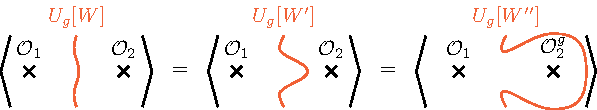
\includegraphics[width=4.16667in,height=\textheight]{index_files/mediabag/figures/Op_action.pdf}

}

\caption{\label{fig-op-action}The topological operator \(U_g[W]\) should
be invariant under a continuous deformation and also implement the
symmetry action.}

\end{figure}

The idea of the construction is
``\emph{cutting-and-gluing-with-twist}''. That is, we first divide the
spacetime \(M\) into two parts: \(M_\stdim = M_L \cup_W M_R\) with
shared boundary \(W\) (see Figure~\ref{fig-cut-M}. We take the
orientation of \(W\) so that \(\partial M_L = -\partial M_R = W\). ). We
also separate the scalar field \(\phi\) into two sets of fields:
\(\phi_L(x)\) for \(x \in M_L\) and \(\phi_R(x)\) for \(x \in M_R\).
Then, we glue the two regions and fields on those back together, with
the twisted identification: \[
\phi_L|_W = \phi_R^{g^{-1}}|_W.
\]

\begin{figure}[t]

{\centering 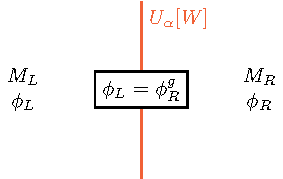
\includegraphics[width=2.39583in,height=\textheight]{index_files/mediabag/figures/ManifoldSplit.pdf}

}

\caption{\label{fig-cut-M}The cutting and twisted gluing, implementing
the topological operator \(U_g[W]\).}

\end{figure}

In path-integral, this construction can be implemented as follows:

\begin{tcolorbox}[enhanced jigsaw, colbacktitle=quarto-callout-important-color!10!white, opacitybacktitle=0.6, bottomrule=.15mm, titlerule=0mm, colframe=quarto-callout-important-color-frame, colback=white, leftrule=.75mm, toprule=.15mm, bottomtitle=1mm, opacityback=0, title=\textcolor{quarto-callout-important-color}{\faExclamation}\hspace{0.5em}{\textsf{Symmetry Topological Operator}}, toptitle=1mm, arc=.35mm, coltitle=black, breakable, left=2mm, rightrule=.15mm]

\begin{equation}\protect\hypertarget{eq-Ug-pathintegral}{}{
\begin{multlined}
    \langle U_g[W] \cdots \rangle = \int \mathop{\mathcal{D}^{M_L}\phi_L} \mathop{\mathcal{D}^{M_R}\phi_R} \mathop{\mathcal{D}^W\lambda} \cdots\\ \times \exp\left(-S_L[\phi_L]-S_R[\phi_R] - G_W[\lambda,\phi_L,\phi_R,g]\right)
\end{multlined}
}\label{eq-Ug-pathintegral}\end{equation}

\end{tcolorbox}

Here, \(\mathcal{D}^{X}\) denotes the measure for path-integral for a
field defined on a submanifold \(X\) of the spacetime \(M\), and
\(S_{L,R} = \int_{M_{L,R}}\mathcal{L}(\phi_{L,R})\) are actions on the
submanifold \(M_{L,R}\), and ``\(\cdots\)'' represents additional
insertions of operators. In addition, the ``gluing'' action \(G_W\) on
the submanifold \(W\) is
\begin{equation}\protect\hypertarget{eq-gluing-action}{}{
\begin{multlined}
    G_W[\lambda,\phi_L,\phi_R,g] = - \imunit \int_W \lambda(\phi_L - \phi_R^{g^{-1}})\vol_W+\int_W s(\phi_M,g).
\end{multlined}
}\label{eq-gluing-action}\end{equation} The heart of the above
expression is that integrating the Lagrange multiplier \(\lambda\) out
gives the ``delta functional'':
\begin{equation}\protect\hypertarget{eq-delta-functional}{}{
\
    \int \mathop{\mathcal{D}^W\lambda} \exp\left(\imunit \int_W \lambda (\phi_L-\phi^{g^{-1}}_R)\vol_W\right)
     = \prod_{x\in W}\delta(\phi_L(x) - \phi_R^{g^{-1}}(x)),
}\label{eq-delta-functional}\end{equation} which should implement
Figure~\ref{fig-cut-M}. Before studying the operator \(U_g[W]\), we
should study the \emph{trivial} case where the symmetry transformation
\(g\) is the identity map \(g=\id\).

\hypertarget{sec-trivial-scalar}{%
\section{Identity Wall}\label{sec-trivial-scalar}}

When \(g=\id\), the operator \(U_{g=\id}[W]\) should be \emph{trivial}.
That is, we have
\begin{equation}\protect\hypertarget{eq-identity-wall}{}{
\langle \id[W] \cdots \rangle = \langle \cdots \rangle.
}\label{eq-identity-wall}\end{equation} We call the codimension-1
operator \(\id[W]\) with this property \textbf{identity wall}. It can
also be called \textbf{transparent wall} or like that. Expanding
Equation~\ref{eq-identity-wall}, the following equation should hold:
\begin{equation}\protect\hypertarget{eq-trivial-scalar}{}{
\begin{multlined}
    \int \mathop{\mathcal{D}^M\phi} \exp(-S) \cdots=
    \int \mathop{\mathcal{D}^{M_L}\phi_L} \mathop{\mathcal{D}^{M_R}\phi_R} \mathop{\mathcal{D}^W\lambda} \\ \times \exp\left(-S_L-S_R+\imunit \int_W \lambda(\phi_L - \phi_R)\vol_W\right)\cdots.\\ 
\end{multlined}
}\label{eq-trivial-scalar}\end{equation}

The point is that the difference between giving a field \(\phi\) and
giving a pair of fields \((\phi_L,\phi_R)\) is that the latter is not
constrained to be continuous across \(W\). On the right-hand side it is
rather enforced by integrating out \(\lambda\) because of
Equation~\ref{eq-delta-functional}.

\begin{tcolorbox}[enhanced jigsaw, colbacktitle=quarto-callout-tip-color!10!white, opacitybacktitle=0.6, bottomrule=.15mm, titlerule=0mm, colframe=quarto-callout-tip-color-frame, colback=white, leftrule=.75mm, toprule=.15mm, bottomtitle=1mm, opacityback=0, title=\textcolor{quarto-callout-tip-color}{\faLightbulb}\hspace{0.5em}{\textsf{Continuity of fields in ``exotic'' QFTs and subsystem symmetry}}, toptitle=1mm, arc=.35mm, coltitle=black, breakable, left=2mm, rightrule=.15mm]

Here we assumed that the path integral \(\int\mathcal{D}^M\phi\) should
be over the \emph{continuous} fields. The reason for this is that the
standard kinetic term would diverge in the limit where the filed
\(\phi\) becomes discontinuous.

This assumption, however, does not apply to QFTs with higher-derivative
kinetic terms. Examples of such exotic QFTs (without relativistic
symmetry) includes tensor gauge theories (see e.g.
\autocite{Pretko:2020cko,Seiberg:2020bhn}). In these theories a field
\emph{can} be discontinuous, but some of higher derivatives are
constrained to scale correctly with respect to the ratio of the lattice
size and the system size. In such cases the construction of the trivial
operator should differ. \emph{KO does not know how to describe it
because of the UV/IR mixing and totally confused}.

These QFTs describes what is called the \textbf{fracton phases} of
matter, which does not have emergent continuous rotational symmetry in
the IR. And the models typically posses \textbf{subsytemsymmetries},
whose corresponding operator is not totally topological. Existence of
the new kind of symmetry lacked in standard relativistic systems would
be related to the fact that the identy wall looks different from the
first place.

\end{tcolorbox}

It is instructive to study the equation of motions (EOMs) on the right
hand side of Equation~\ref{eq-trivial-scalar}. The EOM with respect to
\(\lambda\) simply states \(\phi_L(x) = \phi_R(x)\) for \(x\in W\). The
surface term of Euler-Lagrange equation for \(\phi_L\) and \(\phi_R\)
gives \[
    \left.\frac{\delta \mathcal{L}[\phi_L]}{\delta \mathop{d\phi_L}}\right|_W = \lambda \vol_W = \left. \frac{\delta \mathcal{L}[\phi_R]}{\delta \mathop{d \phi_R}}\right|_W.
\] If \(W\) is spacelike, or we regard the direction perpendicular to
\(W\) as the imaginary time in Euclidean signature, this enforces that
the canonical momentum also be continuous across \(W\).

\begin{tcolorbox}[enhanced jigsaw, colbacktitle=quarto-callout-note-color!10!white, opacitybacktitle=0.6, bottomrule=.15mm, titlerule=0mm, colframe=quarto-callout-note-color-frame, colback=white, leftrule=.75mm, toprule=.15mm, bottomtitle=1mm, opacityback=0, title=\textcolor{quarto-callout-note-color}{\faInfo}\hspace{0.5em}{\textsf{Locality}}, toptitle=1mm, arc=.35mm, coltitle=black, breakable, left=2mm, rightrule=.15mm]

Equation~\ref{eq-trivial-scalar} expresses the \textbf{locality} of the
path-integral. We can use the same procedure to decompose the
path-integral \(\int \mathcal{D}^M{\phi}\) on \(M\) into path-integrals
on local patches like \(\int \prod_i\mathcal{D}^{V_i}\phi_i\) (comes
with many Lagrange multipliers). Here \(\bigcup_i V_i =M\) and
\(V_i \cap V_j\) has codimension 1 in \(M\) if not empty.

Indeed, in the context of topological quantum field theory (TQFT), a
similar \textbf{cutting-and-gluing} axiom is hired by the Atiyah-Segal
formulation of topological quantum field theory and later Lurie's
cobordism hypothesis \autocite{Lurie} established the relation between
it and the locality.

Although in this lecture we satisfy ourselves with the formal
non-rigorous treatment of path-integrals, deeper understanding of
locality in non-topological QFT is strongly desired, and there are some
promising results e.g.~in \autocite{GradyPavlov1}.

\end{tcolorbox}

\begin{tcolorbox}[enhanced jigsaw, colbacktitle=quarto-callout-tip-color!10!white, opacitybacktitle=0.6, bottomrule=.15mm, titlerule=0mm, colframe=quarto-callout-tip-color-frame, colback=white, leftrule=.75mm, toprule=.15mm, bottomtitle=1mm, opacityback=0, title=\textcolor{quarto-callout-tip-color}{\faLightbulb}\hspace{0.5em}{\textsf{A comment about fermion}}, toptitle=1mm, arc=.35mm, coltitle=black, breakable, left=2mm, rightrule=.15mm]

Because we do not plan to talk about fermion in this lecture, we comment
on what will differ in the case of fermions.

In the scalar field theory, we impose the continuity of the ``position''
variables (in analytical-mechanical sense) \(\phi\), then the continuity
of the momentum variables follows by EOM.

In a chiral fermion theory, as its kinetic term involves only one
derivative, momentum and position variables cannot typically be possible
in a way preserving Lorentz or global chiral symmetry. Thus, the
``cutting'' have to induce an apparent violation of invariance under the
Lorentz or the other symmetry, which is a way of seeing the
gravitational and global symmetry anomaly. The precise understanding of
this perspective is remained to be open in this lecture (and not in the
literature as far as the author knows).

\end{tcolorbox}

\hypertarget{symmetry-action-and-ward-takahashi-identity}{%
\section{Symmetry Action and Ward-Takahashi
identity}\label{symmetry-action-and-ward-takahashi-identity}}

Let us turn to the non-trivial operator
Equation~\ref{eq-Ug-pathintegral} and check the property depicted in
Figure~\ref{fig-op-action}. In order to do it, start from the correlator
where \(U_g\) is inserted along \(W=W_1\) and the trivial operator
\(\id\) along \(W''=W_2\) in Figure~\ref{fig-op-action}. (Here we only
talk about the equality connecting the leftmost and rightmost figures of
Figure~\ref{fig-op-action}. For the middle one the argument is the same.
We also renamed the manifolds for the later convenience.) Therefore we
split the manifold \(M\) into three regions \(M_L,M_M,M_R\), and also
the field \(\phi\) into \(\phi_L,\phi_M,\phi_R\). Then to show the
equality in Figure~\ref{fig-op-action}, we perform the change of the
variable \(\widetilde{\phi}_M = \phi_M^{g^{-1}}\) : \[
\begin{aligned}
    &\langle \mathcal{O}_1 U_g[W_1] \mathcal{O}_2 \rangle = \langle \mathcal{O}_1 U_g[W_1] \mathcal{O}_2 \id[W_2] \rangle \\
     &= \int \prod_{i=L,M,R}\mathop{\mathcal{D}^{M_i}\phi_i} \mathop{\prod_{a=1,2}\mathcal{D}^{W_a} \lambda_a} e^{-S_L[\phi_L]-S_M[\phi_M]-S_R[\phi_R]}\mathcal{O}_1[\phi_L] \mathcal{O}_2[\phi_M]
     \\ 
     &\times \exp\left(-G_{W_1}[\lambda_1,\phi_L,\phi_M,g]-G_{W_2}[\lambda_2,\phi_M,\phi_R,\id]\right)\\
     &= \int \prod_{i=L,M,R}\mathop{\mathcal{D}^{M_i}\phi_i} \mathop{\prod_{a=1,2}\mathcal{D}^{W_a}\lambda_a} e^{-S_L[\phi_L]-S_M[\widetilde\phi_M^g]-S_R[\phi_R]}\mathcal{O}_1[\phi_L] \mathcal{O}_2[\widetilde\phi_M^g]
     \\ 
     &\times \exp\left(-G_{W_1}[\lambda_1,\phi_L,\widetilde\phi_M,\id]-G_{W_2}[\lambda_2,\widetilde{\phi}_M^g,\phi_R,\id]\right)\\ 
     &\times \exp\left( + \int_W s(\phi_L,g) \right)\\ 
     &= \int \prod_{i=L,M,R}\mathop{\mathcal{D}^{M_i}\phi_i} \mathop{\prod_{a=1,2}\mathcal{D}^{W_a}\lambda_a} e^{-S_L[\phi_L]-S_M[\widetilde\phi_M^g]-S_R[\phi_R]}\mathcal{O}_1[\phi_L] \mathcal{O}_2^g[\widetilde\phi_M]
     \\ 
     &\times \exp\left(-G_{W_1}[\lambda_1,\phi_L,\widetilde\phi_M,\id]-G_{-W_2}[\lambda_2,\phi_R,\widetilde{\phi}_M,g^{-1}]\right)\\ 
     &\times \exp\left( + \int_{W_1} s(\phi_M,g) + \int_{W_2} s(\phi_M,g^{-1})  \right)\\
     &= \int \prod_{i=L,M,R}\mathop{\mathcal{D}^{M_i}\phi_i} \mathop{\prod_{a=1,2}\mathcal{D}^{W_a}\lambda_a} e^{-S_L[\phi_L]-S_M[\widetilde\phi_M]-S_R[\phi_R]}\mathcal{O}_1[\phi_L] \mathcal{O}_2^g[\widetilde\phi_M]
     \\ 
     &\times \exp\left(-G_{W_1}[\lambda_1,\phi_L,\widetilde\phi_M,\id]-G_{-W_2}[\lambda_2,\phi_R,\widetilde{\phi}_M,g^{-1}]\right)\\
     &= \langle \mathcal{O}_1 \id[W_1] \mathcal{O}_2 U_{g^{-1}}[-W_2]. \rangle
\end{aligned}
\] In the second to last equality we used
Equation~\ref{eq-Lagrangian-inv} and in the last equality we assumed
that the path-integral measure is invariant:
\begin{equation}\protect\hypertarget{eq-measure-inv}{}{\mathcal{D}\phi_M = \mathcal{D}\phi_M^g.
}\label{eq-measure-inv}\end{equation} Lastly, from
Equation~\ref{eq-delta-functional} we get \(U_{g^{-1}}[-W] = U_g[W]\),
so we obtain Figure~\ref{fig-op-action}, that is
\begin{equation}\protect\hypertarget{eq-sym-op-act}{}{
\langle \mathcal{O}_1 U_g[W_1] \mathcal{O}_2 \rangle = \langle \mathcal{O}_1 \mathcal{O}_2^g U_g[W_2] \rangle.
}\label{eq-sym-op-act}\end{equation}

We note that we can also get the following equation in the same way as
above: \begin{equation}\protect\hypertarget{eq-bubble}{}{
\langle \mathcal{O}_1 \mathcal{O}_2 \cdots \rangle = \langle U_g[W_0] \mathcal{O}_1 \mathcal{O}_2^g \cdots \rangle,
}\label{eq-bubble}\end{equation}

when \(W_0\) encloses a compact region of \(M\) and contains no
operator. Then, by repeatedly using these equations, we get the
\textbf{Ward-Takahashi identity} (\textbf{FIXME:figure})

\begin{tcolorbox}[enhanced jigsaw, colbacktitle=quarto-callout-important-color!10!white, opacitybacktitle=0.6, bottomrule=.15mm, titlerule=0mm, colframe=quarto-callout-important-color-frame, colback=white, leftrule=.75mm, toprule=.15mm, bottomtitle=1mm, opacityback=0, title=\textcolor{quarto-callout-important-color}{\faExclamation}\hspace{0.5em}{\textsf{Ward-Takahashi Identity}}, toptitle=1mm, arc=.35mm, coltitle=black, breakable, left=2mm, rightrule=.15mm]

\begin{equation}\protect\hypertarget{eq-Ward-Takahashi}{}{
\begin{aligned}
\langle \mathcal{O}_1 \mathcal{O}_2 \cdots \mathcal{O}_N \rangle
&= 
\langle U_g[W_0] \mathcal{O}_1 \mathcal{O}_2 \cdots \mathcal{O}_N \rangle\\
&= 
\langle \mathcal{O}_1^g U_g[W_1] \mathcal{O}_2 \cdots \mathcal{O}_N \rangle\\
&= 
\langle \mathcal{O}_1^g  \mathcal{O}_2^g \cdots \mathcal{O}_N^g U_g[W_N] \rangle\\
&= 
\langle \mathcal{O}_1^g  \mathcal{O}_2^g \cdots \mathcal{O}_N^g\rangle,
\end{aligned}
}\label{eq-Ward-Takahashi}\end{equation} where \(W_i\) encloses the
operators \(\mathcal{O}_1 \cdots \mathcal{O}_i\), and at the last step
we collapsed \(U_g[W_N]\) towards the infinity (or whatever point if
\(M\) is compact).

\end{tcolorbox}

Of course we could get the same result by considering global change of
variable \(\widetilde{\phi} = \phi^{g^{-1}}\), the point is that, once
the existence of topological operator is established, the derivation of
the Ward-Takahashi identity can be done in the same way, even if the
symmetry does not come from field transformation.

\textbf{FIXME:explain about the selection rule}

\begin{tcolorbox}[enhanced jigsaw, colbacktitle=quarto-callout-tip-color!10!white, opacitybacktitle=0.6, bottomrule=.15mm, titlerule=0mm, colframe=quarto-callout-tip-color-frame, colback=white, leftrule=.75mm, toprule=.15mm, bottomtitle=1mm, opacityback=0, title=\textcolor{quarto-callout-tip-color}{\faLightbulb}\hspace{0.5em}{\textsf{Mixed-gravitational anomaly}}, toptitle=1mm, arc=.35mm, coltitle=black, breakable, left=2mm, rightrule=.15mm]

The symmetry we discuss here does not suffer from anomaly and the
Ward-Takahashi idendity (Equation~\ref{eq-Ward-Takahashi}) follows. If
we instead consider the topological operator corresponding to a symmetry
with mixed-gravitational anomaly, the invariance of the measure
(Equation~\ref{eq-measure-inv}) does not necessarily hold when \(M_M\)
does not have the topology of a ball, and likewise
Equation~\ref{eq-bubble} can fail when \(W_0\) is not a ball. Thus, on a
spacetime with non-trivial topology (other than \(\mathbb{R}^4\) or
\(S^4\)), (Equation~\ref{eq-Ward-Takahashi}) might fail at the last
equality, while (by choosing \(W_0\) to be a ball) other steps goes
through. The failure is by a phase depending on topology of the
spacetime, and has an interesting consequences of this discussed in
\autocite{Cordova:2019jqi}.

\end{tcolorbox}

\hypertarget{relation-to-noether-charge}{%
\section{Relation to Noether Charge}\label{relation-to-noether-charge}}

Here we show the relation Equation~\ref{eq-Noether-approx} of the
topological operator \(U_g[W]\) to the conventional Noether charge. This
can be done by applying the change of variable
\(\widetilde{\phi_R} = \phi^{\id - \alpha f(x_n)}_R\) to
Equation~\ref{eq-Ug-pathintegral}, where \(f(x_n,\delta)\) is a function
of the coordinate \(x_n\) perpendicular to \(W\) and one positive
parameter \(\delta\) and satisfies \(f(0) = 1\) and
\(f(x_n>\delta) =0\). Then we take \(\delta\to 0\) limit and compare.
\textbf{FIXME:write equations}

\bookmarksetup{startatroot}

\hypertarget{sec-compact-boson}{%
\chapter{Compact Boson}\label{sec-compact-boson}}

Here we consider \emph{compact} boson, where the field \(\phi\) is real
and subject to the identification \[
\phi(x) \cong \phi(x) + 2\pi.
\] We take the Lagrangian to be \[
\mathcal{L} = \frac{R^2}{4\pi}\int_M \mathop{d\phi} \wedge \mathop{*}\mathop{d\phi}.
\] We can normalize the field \(\phi\) so that it has the kinetic term
with a fixed coefficient, in which case the normalized field has a
periodicity radius proportional to \(R\).

The theory has the shift (or ``momentum'') \(\U(1)\) symmetry \[
\phi^\alpha = \phi + \alpha 
\] with identification of the parameter \(\alpha \cong \alpha + 2\pi\).
One can add a periodic potential \(V(\phi)\) and restrict oneself to a
discrete symmetry preserving the potential.

In addition to the shift symmetry, the system has other generalized
symmetries:

\begin{enumerate}
\def\labelenumi{\arabic{enumi}.}
\tightlist
\item
  \textbf{winding} \(\U(1)\) (\(\stdim-2\))-form symmetry
  \autocite{Gaiotto:2014kfa}, and
\item
  when \(\stdim=2\) and \(R^2\) is rational, there exists a
  \textbf{T-duality} symmetry that is in general \emph{non-invertible}
  \autocites{Choi:2021kmx}{Niro:2022ctq}{Cordova:2023ent,Nagoya:2023zky}.
\end{enumerate}

The purpose of this section is to understand these generalized
symmetries, but before that we review the shift symmetry.

\hypertarget{trivial-operator-and-shift-symmetry-operator}{%
\section{Trivial Operator and Shift Symmetry
Operator}\label{trivial-operator-and-shift-symmetry-operator}}

We start from the identity operator \(\id[W^{\stdim-1}]\) that cuts and
glues the path-integral. The construction is almost the same as before,
but when we glue the fields \(\phi_L\) and \(\phi_R\) along
\(W^{\stdim-1}\), the gluing can be up to a integer multiple of
\(2\pi\): \[
    \phi_L(x) = \phi_R(x) + 2\pi n 
\] with an integer \(n\) (assuming \(W^{\stdim-1}\) is connected).
Therefore, the gluing part of the path-integral is \[
\id[W^{\stdim-1}] = \sum_{n\in\mathbb{Z}}\int \mathcal{D}^{W^{\stdim-1}}\lambda \exp\left(\imunit\int_{W^{\stdim-1}} \lambda\left(\phi_L-\phi_R - 2\pi n\right)\right)\vol_{W^{\stdim-1}}.
\] We can sum \(n\) out to restrict \(\lambda\) to satisfy \[
    \int_{W^{\stdim-1}}\lambda \vol_{W^{\stdim-1}} \in \mathbb{Z}.
\] An integration over such lambda can be replaced by integration in
terms of \((\stdim-2)\)-form \(\U(1)\) gauge field \(V\) with \[
\mathop{dV} = 2\pi \lambda\vol_{W^{\stdim-1}}.
\] Therefore the identity operator can be written as\footnote{We assume
  that the integration should be done over \emph{gauge equivalent
  classes} of \(V\). In other words the gauge fixing procedure is
  implicit in this lecture.}
\begin{equation}\protect\hypertarget{eq-identity-compact-boson}{}{
    \id[{W^{\stdim-1}}] = \int \mathcal{D}^{W^{\stdim-1}}V \exp\left(\frac{\imunit}{2\pi}\int_{W^{\stdim-1}} \mathop{dV}\left(\phi_L-\phi_R\right)\right).
}\label{eq-identity-compact-boson}\end{equation}

\begin{tcolorbox}[enhanced jigsaw, colbacktitle=quarto-callout-note-color!10!white, opacitybacktitle=0.6, bottomrule=.15mm, titlerule=0mm, colframe=quarto-callout-note-color-frame, colback=white, leftrule=.75mm, toprule=.15mm, bottomtitle=1mm, opacityback=0, title=\textcolor{quarto-callout-note-color}{\faInfo}\hspace{0.5em}{\textsf{\(p\)-form gauge field}}, toptitle=1mm, arc=.35mm, coltitle=black, breakable, left=2mm, rightrule=.15mm]

A \(p\)-form gauge field \(V\) is \emph{locally} (i.e.~in a patch)
\(p\)-form, but \(V\) is not necessarily a \emph{global} \(p\)-form and
\(\mathop{dV}\) rather satisfy
\(\int_{\Sigma_{p+1}}\mathop{dV}\in 2\pi \mathbb{Z}\) for any \(p+1\)
dimensional submanifold.

If a reader is not familiar with this concept, one can assume
\(\stdim = 2,3\). When \(\stdim=3\), \(V\) is a usual (one-form) abelian
gauge field, whose magnetic flux is quantized, while when \(\stdim =2\),
\(V\) is a periodic scalar field. About higher-form gauge field, a
motivated reader can consult e.g.~\textcite{Hsieh:2020jpj}.

\end{tcolorbox}

Now the topological operator for the shift symmetry is simply
\begin{equation}\protect\hypertarget{eq-shift-compact-boson}{}{
    U_\alpha^\text{shift}[{W^{\stdim-1}}] = \int \mathcal{D}^{W^{\stdim-1}}V \exp\left(\frac{\imunit}{2\pi}\int_{W^{\stdim-1}} \mathop{dV}\left(\phi_L-\phi_R + \alpha\right)\right).
}\label{eq-shift-compact-boson}\end{equation}

\hypertarget{winding-symmetry}{%
\section{Winding Symmetry}\label{winding-symmetry}}

The compact boson theory has another topological operator of dimension 1
(codimension \(\stdim-1\)), which is simply
\begin{equation}\protect\hypertarget{eq-winding-op}{}{
U^\text{winding}_\alpha[\gamma^1] = \exp\left(\imunit\alpha \int_{\gamma^1}\frac{\mathop{d\phi}}{2\pi}\right).
}\label{eq-winding-op}\end{equation} Given the periodicity, the integral
\(\int_{\gamma^1}\mathop{d\phi}\) for a closed \(\gamma^1\) takes a
value in \(2\pi \mathbb{Z}\), and therefore the operator is invariant
against deformation of \(\gamma^1\). This also indicates that the
parameter \(\alpha\) is \(2\pi\) periodic. According to
Table~\ref{tbl-sym-classes}, this topological operator should define a
\(\U(1)\) \(p\)-form symmetry with \(p=(\stdim-2)\), called the
\textbf{winding symmetry}.

What are the operators \emph{charged} under the symmetry? When
\(p \ge 1\) (\(\stdim\ge 3\)), the operator Equation~\ref{eq-winding-op}
cannot act on a local (point) operator, because the one-dimensional
submanifold \(\gamma^1\) can always be deformed one configuration to
another without colliding with a point. On the other hand, it can
potentially act on a \(p\)-dimensional extended operator.
\textbf{FIXME:figure!!}.

However, the construction of a charged operator is a bit tricky. A way
of doing it is to first insert the identity operator
Equation~\ref{eq-identity-compact-boson}, then utilize the field \(V\)
on the identity operator to defing an operator charged under
Equation~\ref{eq-winding-op}. Concretely, the (non-topological) operator
with winding charge \(n\) can be constructed as
\begin{equation}\protect\hypertarget{eq-dual-op}{}{
\langle \mathcal{O}^\text{winding}_n[\Sigma^{D-2}] \rangle
= \int \mathcal{D}^{W^{\stdim-1}}V \exp\left(\frac{\imunit}{2\pi}\int_{W^{\stdim-1}} \mathop{dV}\left(\phi_L-\phi_R\right)+\imunit n \int_{\Sigma^{\stdim-2}}V\right).
}\label{eq-dual-op}\end{equation} Here, we take arbitrary
\(W^{\stdim-1}\) that contains \(\Sigma^{\stdim-2}\), and the correlator
is independent of the choice. The coefficient \(n\) has to be an integer
for \(\int_{\Sigma^{D-1}}\) to be invariant under global gauge
transformations.

The operator Equation~\ref{eq-dual-op} is often defined as a
``disorder'' operator that enforces singular behavior. Here we see the
explicit construction of such by \emph{integrating in} the Lagrange
multiplier \(V\) on \(W^{\stdim-1}\).

\begin{tcolorbox}[enhanced jigsaw, colbacktitle=quarto-callout-note-color!10!white, opacitybacktitle=0.6, bottomrule=.15mm, titlerule=0mm, colframe=quarto-callout-note-color-frame, colback=white, leftrule=.75mm, toprule=.15mm, bottomtitle=1mm, opacityback=0, title=\textcolor{quarto-callout-note-color}{\faInfo}\hspace{0.5em}{Note}, toptitle=1mm, arc=.35mm, coltitle=black, breakable, left=2mm, rightrule=.15mm]

Note that the topological operator Equation~\ref{eq-Ug-pathintegral} is
also of disorder-type; it enforces a jump of the field across \(W\). It
is curious that, for symmetry of field transformation, the
charg\emph{ed} operators are direct to construct, while the symmetry
topological operator was somewhat tedious to do; and it is opposite for
the winding symmetry, or more generally topological charges.

\begin{longtable}[]{@{}lll@{}}
\toprule\noalign{}
& Field transformation & Topological charge \\
\midrule\noalign{}
\endhead
\bottomrule\noalign{}
\endlastfoot
Charged operator & not disorder & disorder \\
Topological operator & disorder & not disorder \\
\end{longtable}

One aim of this lecture is to demystify the ``disorder'' operators --
they can be explicitly written in terms of correct set of Lagrange
multipliers -- so that one can talk about the two types of the symmetry
in a unified way.

\end{tcolorbox}

\textbf{FIXME:derivation of the charge, from EOM of V}

Now the Ward-Takahashi identity Equation~\ref{eq-Ward-Takahashi}
formally follows from the topological-ness of
Equation~\ref{eq-winding-op}. Explicitly, we have \[
\langle \prod_i \mathcal{O}^\text{winding}_{n_i}(x_i)\rangle 
=
\langle \prod_i e^{\imunit \alpha n_i} \mathcal{O}^\text{winding}_{n_i}(x_i)\rangle 
\] for any \(\alpha\). And thus the both sides vanish unless
\(\sum n_i = 0\).

\hypertarget{mixed-anomaly-between-shift-and-winding-symmetry}{%
\section{Mixed Anomaly between Shift and Winding
Symmetry}\label{mixed-anomaly-between-shift-and-winding-symmetry}}

\hypertarget{intersection}{%
\subsection{Intersection}\label{intersection}}

Having explicit descriptions of topological operators enables us to
directly compute \textbf{quantum anomaly} (often called 't Hooft
anomaly) of the symmetries. This is because, from a modern perspective,
the anomaly is a subtlety arises when symmetry operators collide. Here
we observe one example of anomaly -- the mixed anomaly between the shift
and winding symmetry in the compact boson theory -- explicitly from the
topological operator perspective. For a general theory about anomaly and
topological operator, readers can consult other resources, e.g.
\textcite{TachikawaTasi}.

Let us study the intersection of \(U_\alpha^\text{shift}[W^{\stdim-1}]\)
(Equation~\ref{eq-shift-compact-boson}) and
\(U_\beta^\text{winding}[\gamma^1]\) (Equation~\ref{eq-winding-op}).
\textbf{FIXME:figure} The shift symmetry operator divides \(\gamma^1\)
into \(\gamma^1_L\) and \(\gamma^1_R\), and the winding operator thus
now, naively, look like \[
\begin{aligned}
U^\text{shift}_\alpha U^\text{winding}_\beta[\gamma^1] &\stackrel{\text{naive}}{=} U^\text{shift}_\alpha \exp\left(\imunit\beta \left(\int_{\gamma^1_L}\frac{\mathop{d\phi_L}}{2\pi} + \int_{\gamma^1_R}\frac{\mathop{d\phi_R}}{2\pi}\right)\right)\\
& \sim U^\text{shift}_\alpha \exp\left(\imunit\beta/2\pi (\phi_L(x_0) - \phi_R(x_0)) \right),
\end{aligned}
\] where in the second line, \(\sim\) refers to the contribution local
to the intersection point \(x_0\) (i.e.~we ignored the contribution from
the other ends of \(\gamma^1_L\) and \(\gamma^1_R\) far from
\(W^{\stdim-1}\)). However, the shift symmetry defect enforces
\(\phi_L = \phi_R - \alpha \mod 2\pi\), but the local contribution at
\(x_0\) \emph{depends} on \(\phi_L-\phi_R \mod 2\pi\). Therefore the
naive definition of intersected operator is not well-defined (or, it
becomes zero if we average over the branches of
\(\phi_L(x_0) -\phi_R(x_0)\)).

A way to define the intersection is to abandon the periodicity of either
of \(\alpha\) or \(\beta\). If we regard \(\alpha\) to be in
\(\mathbb{R}\) and not \(\mathbb{R}/2\pi\mathbb{Z}\), we can modify the
above naive definition to be \[
\begin{aligned}
U^\text{shift}_\alpha U^\text{winding}_\beta[\gamma^1] &\stackrel{\text{def1}}{=} U^\text{shift}_\alpha \exp\left(\imunit\beta \left(\int_{\gamma^1_L}\frac{\mathop{d\phi_L}}{2\pi} + \int_{\gamma^1_R}\frac{\mathop{d\phi_R}}{2\pi} + \{\alpha/2\pi\}\right)\right)\\
& \sim U^\text{shift}_\alpha \exp\left(\imunit\beta [\alpha/2\pi] \right),
\end{aligned}
\] where \([r]\) is the integer part of a real number \(r\), and
\(\{r\}= r-[r]\). With this definition, or regularization, of the
intersection, \(\alpha\) is no longer periodic, but \(\beta\) is kept
periodic. One can do other regularizations where \(\alpha\) is periodic
but \(\beta\) is not, or just abandon both of periodicity, but cannot
save both.

This incompatibility of periodicity, or the group multiplication law,
when topological operators intersects is the hallmark of anomaly.

\hypertarget{group-cohomology}{%
\subsection{Group Cohomology}\label{group-cohomology}}

The incompatibility above is better characterized as a group cohomology
(or its generalization to a higher-group). Here we see how to
characterize the mixed anomaly of the compact boson in 1+1d as a group
cohomology element. (Here we do not delve into the general theory of
group cohomology. See e.g.~\textcite{TachikawaTasi}).

In 1+1d, both \(U^\text{shift}_\alpha\) and \(U^\text{winding}_\beta\)
are line operators. Both operators are \(2\pi\) periodic in its
parameters, when intersection between them are absent. A more precise
statement that applies even with intersections is that
\(U^\text{shift}_\alpha\) and \(U^\text{shift}_{\alpha+2\pi}\) can be
connected with an invertible topological line-changing operator or a
\emph{line-isomrphism} operator for short\footnote{In the language of
  category theory, such an invertible topological line-changing operator
  defines an \emph{isomorphism} between the lines. In (higher)-category
  theory it is important to to distinguish being isomorphic from being
  ``the same'', and in this context physically it means that we remember
  the total derivative terms on the line.}: \[
 \exp\left(\frac{\imunit}{2\pi} \int^\square \mathop{dV}(\phi_L-\phi_R -\alpha)  + \imunit V(\square)  + \frac{\imunit}{2\pi} \int_\square \mathop{dV}(\phi_L-\phi_R -\alpha+2\pi)  \right)
\] where \(\square\) denotes the point connecting two line operators.
Note that the winding operator \(e^{\imunit V(\square)}\) is precisely
cancelled when the integral in the last term is evaluated, and thus the
junction operator is topological. The existence of its inverse is also
manifest.

See also Figure~\ref{fig-line-isom}

\begin{figure}

\begin{minipage}[t]{0.50\linewidth}

{\centering 

\raisebox{-\height}{

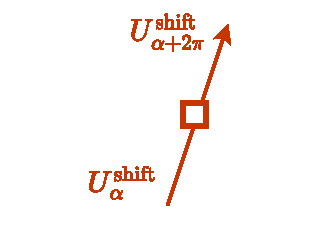
\includegraphics{figures/shift_2pi_isom.pdf}

}

}

\end{minipage}%
%
\begin{minipage}[t]{0.50\linewidth}

{\centering 

\raisebox{-\height}{

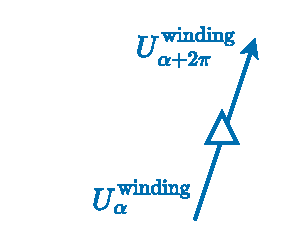
\includegraphics{figures/winding_2pi_isom.pdf}

}

}

\end{minipage}%

\caption{\label{fig-line-isom}Line-isomorphism operators.}

\end{figure}

We let the composition of the two lines be denoted by
\(U_{\alpha,\beta} = U^\text{shift}_\alpha U^\text{winding}_\beta\).
Note that here we already has made a choice -- that we put the shift
operator to the left of the winding operator in \(U_{\alpha,\beta}\).

\hypertarget{t-duality}{%
\section{T-duality}\label{t-duality}}

The compact boson in \(\stdim=2\)-dimensions famously has
\emph{T-duality}.

The T-duality is equivalence between the compact boson with radius \(R\)
and radius \(\frac{1}{R}\), and maps the shift (or momentum) symmetry of
one side to the winding symmetry of the other side, and vise versa. Note
that this makes sense because in \(\stdim=2\) the winding symmetry is a
0-form symmetry.

When the radius is the self-dual radius \(R=1\), the duality becomes a
(conventional) \(\mathbb{Z}_2\) symmetry, which is a part of the larger
emergent \(\SU(2)\) symmetry.

In this section we study

\begin{enumerate}
\def\labelenumi{\arabic{enumi}.}
\tightlist
\item
  the explicit construction of the T-duality topological interface
  connecting radius \(R\) and \(1/R\) theories
  \autocite{Kapustin:2009av}, and
\item
  its generalization giving \textbf{non-invertible} symmetry
  (i.e.~self-dual topological interface) at \(R=\sqrt{N}\) for an
  integer \(N\).
\end{enumerate}

The latter can further be generalized to the case of rational \(R^2\)
\autocite{Niro:2022ctq,Cordova:2023ent}.

\hypertarget{t-duality-topological-interface}{%
\subsection{T-duality topological
interface}\label{t-duality-topological-interface}}

Here we study the T-duality topological interface connecting two compact
boson theories in \(\stdim=2\)-dimensions; with radius \(R\) and radius
\(1/R\). \textbf{FIXME:figure!} When \(R=1\), the interface is a
topological operator within the same thoery, and thus defines a
symmetry. In this case it turns out a \(\mathbb{Z}_2\) symmetry, known
to be contained in the larger \(\SU(2)\) enhanced symmetry.

According to \autocite{Kapustin:2009av}, the partition functino
involving the interface is
\begin{equation}\protect\hypertarget{eq-T-interface}{}{
\begin{multlined}
\langle \mathcal{O}_L \mathcal{I}^\text{T}_1[W] \mathcal{O}_R  \rangle= 
\int \mathop{\mathcal{D}^{M_L}\phi_L}\mathop{\mathcal{D}^{M_R}\phi_R}
\mathcal{O}_L[\phi_L]\mathcal{O}_R[\phi_R]\\
\exp\left(-\frac{R^2}{4\pi}\int_{M_L}\mathop{d\phi_L}*\mathop{d\phi_L}
-\frac{\imunit}{2\pi}\int_W \phi_L\mathop{d\phi_R}
-\frac{1}{4\pi R^2}\int_{M_R}\mathop{d\phi_R}*\mathop{d\phi_R}\right).
\end{multlined}
}\label{eq-T-interface}\end{equation} For simplicity let us take
\(\mathcal{O}_R =1\), and \(M_R\) be a compact region in the spacetime.
In this case, we expect the supposed topological-ness implies \[
\langle \mathcal{O}_L \mathcal{I}_1^\text{T}[W]\rangle = \langle \mathcal{O}_L \rangle.
\] To show this, we replace the variable \(\phi_R\) with
\(F_R = d\phi_R\) by \[
\int \mathcal{D}\phi_R = \int \mathop{\mathcal{D}F_R} \mathop{\mathcal{D}\widetilde{\phi}_R}
\exp\left(\frac{\imunit}{2\pi} \int_{M_R}\widetilde{\phi}_R \mathop{dF_R}\right),
\] where the periodic scalar \(\widetilde{\phi}_R\) is the Lagrange
multiplier enforcing the closedness and the quantization of
\(F_R = d\phi_R\). Substituting this into Equation~\ref{eq-T-interface},
the EOMs with respect to \(F_R\) are
\begin{equation}\protect\hypertarget{eq-EOM-FR-boson}{}{
\begin{aligned}
    \frac{1}{R} *d\phi_R(x) &= \imunit d\widetilde\phi_R(x) \quad \mathop{\text{for}} x \in M_R \\
    \phi_L(x) &= \widetilde{\phi}_R(x) \quad \mathop{\text{for}} x \in W.
\end{aligned}
}\label{eq-EOM-FR-boson}\end{equation} Substituting the former equation
to the Lagrangea of \(\phi_R\), we get \[
    \frac{R^2}{4\pi} \int_{M_R}\mathop{d\widetilde{\phi}_R}*\mathop{d\widetilde{\phi}_R}
\] with is the same as for \(\phi_L\), while the latter of
Equation~\ref{eq-EOM-FR-boson} connects \(\phi_L\) and
\(\widetilde{\phi}_R\) along \(W\). As a whole, we recover the
path-integral over \(M\) resulting in \(\langle \mathcal{O}_L \rangle\).
For a more general topological-ness about local deformation of \(W\) can
be derived in the same way but with more letters.

Now, let us set \(\mathcal{O}_R = \mathcal{O}^\text{winding}_n(x)\) and
see how the topological interface acts on the operator. As the operator
\(\mathcal{O}^\text{winding}_n\) in Equation~\ref{eq-dual-op} is defined
on the trivial surface operator, we have to divide the manifold into
three parts: \(M_L,M_M,m_R\), separated by \(W_1\) and \(W_2\). As the
\(M_L\) and field on it is not going to be relevant, we suppress them in
the following equations. The calculation goes as:

\[
\begin{aligned}
\mathcal{I}_1^\text{T} \mathcal{O}^\text{winding}_n(x)
&= \int \mathop{\mathcal{D}\phi_M}\mathop{\mathcal{D}\phi_R}\mathop{\mathcal{D}^{W_2}V}
\exp\left(-S_M^{1/R}-S_R^{1/R}-\frac{\imunit}{2\pi}\int_{W_1}\phi_L \mathop{d\phi_M}\right)\\
 &\times\exp\left(\frac{\imunit}{2\pi}\int_{W_2}\mathop{dV}(\phi_M-\phi_R) + \imunit n V(x) \right)\\
&= \int \mathop{\mathcal{D}F_M}\mathop{\mathcal{D}F_R}\mathop{\mathcal{D}^{W_2}V}\mathop{\mathcal{D}\widetilde\phi_M}\mathop{\mathcal{D}\widetilde\phi_R}\\
&\times\exp\left(-S_M^{1/R}-S_R^{1/R}-\frac{\imunit}{2\pi}(\int_{W_1}\phi_L \mathop{d\phi_M}-\int_{M_M}\tilde{\phi}_M\mathop{dF_M} - \int_{M_R}\tilde{\phi}_R\mathop{dF_R})\right)\\
 &\times\exp\left(+\frac{\imunit}{2\pi}\int_{W_2}\mathop{V}(F_M-F_R) + \imunit n V(x) \right)
\end{aligned}
\] Now, the EOMs in terms of \(F_M\) and \(F_R\) state \[
\begin{aligned}
    \frac{1}{R} *d\phi_{M,R} &= \imunit d\widetilde\phi_{M,R}(x) \quad \text{on} \;\; M_{M,R}, \\
    \phi_L &= \widetilde{\phi}_M \quad \text{on} \;\; W_1,\\
\tilde{\phi}_M &= V = \tilde{\phi}_R \quad \text{on} \;\; W_2.
\end{aligned}
\] Thus by substituting back we get \textbf{FIXME:check the sign!} \[
\mathcal{I}_1^\text{T}\cdots\mathcal{O}_n^\text{winding} = \mathcal{O}_{\pm? n}^\text{shift}.
\]

In addition, let us calculate \((\mathcal{I}_1[W]^\text{T})^2\). For
this, we insert the defects along parallel submanifolds \(W_1\) and
\(W_2\) and take the limit where the separation of the two shrinks.
\textbf{FIXME:figure} This can be calculated as \[
\begin{aligned}
\mathcal{I}_1^\text{T}[W_1]\mathcal{I}_1^\text{T}[W_2]
&= \int \mathcal{D}^{M_M}\phi_M \exp(-\imunit \int_{W_1} \phi_L d\phi_M - \imunit\int_{W_2} \phi_M d\phi_R)\\
&= \int \mathcal{D}^{W}\phi_M \exp(-\imunit \int_{W} (\phi_L - \phi_R) d\phi_M)\\
&= \id[W],
\end{aligned}
\] where in the second line we collide \(W_1\) and \(W_2\), and noted
that only the mode of \(\phi_M\) constant along the direction
perpendicular to \(W_1\) and \(W_2\) contributes. Therefore, the
T-duality interface squares to the identity. In particular, at \(R=1\),
the self-interface defines an invertible \(\mathbb{Z}_2\) symmetry.

\hypertarget{non-invertible-symmetry-from-t-duality}{%
\subsection{Non-invertible symmetry from
T-duality}\label{non-invertible-symmetry-from-t-duality}}

\textcite{Choi:2021kmx} generalized the Kapustin-Tikhonov T-duality
interface by \textcite{Kapustin:2009av} as
\begin{equation}\protect\hypertarget{eq-TN-interface}{}{
\begin{multlined}
\langle \mathcal{O}_L \mathcal{I}^\text{T}_N[W] \mathcal{O}_R  \rangle= 
\int \mathop{\mathcal{D}^{M_L}\phi_L}\mathop{\mathcal{D}^{M_R}\phi_R}
\mathcal{O}_L[\phi_L]\mathcal{O}_R[\phi_R]\\
\exp\left(-\frac{R^2}{4\pi}\int_{M_L}\mathop{d\phi_L}*\mathop{d\phi_L}
-\frac{\imunit N}{2\pi}\int_W \phi_L\mathop{d\phi_R}
-\frac{N^2}{4\pi R^2}\int_{M_R}\mathop{d\phi_R}*\mathop{d\phi_R}\right).
\end{multlined}
}\label{eq-TN-interface}\end{equation} This interface is a
\emph{self-interface} at \(R=\sqrt{N}\). The same procedure as we did
for \(\mathcal{I}_1\) leads to
\begin{equation}\protect\hypertarget{eq-TN-interface2}{}{
\begin{multlined}
\langle\mathcal{O}_L \mathcal{I}^\text{T}_N[W] \rangle= 
\int \mathop{\mathcal{D}^{M_L}\phi_L}\mathop{\mathcal{D}^{M_R}\phi_R}\mathop{\mathcal{D}^{W}V'}
\mathcal{O}_L[\phi_L]\\
\exp\left(-\frac{R^2}{4\pi}\int_{M_L}\mathop{d\phi_L}*\mathop{d\phi_L}
-\frac{\imunit }{2\pi}\int_W (N \phi_L - \widetilde{\phi}_R)\mathop{dV}
-\frac{R^2}{4\pi N^2}\int_{M_R}\mathop{d\widetilde\phi_R}*\mathop{d\widetilde\phi_R}\right).
\end{multlined}
}\label{eq-TN-interface2}\end{equation} We further rescale the fields as

\[
\begin{aligned}
V' &= NV \\
N \widetilde\phi_R' &= \widetilde\phi_R \mod 2\pi
\end{aligned}
\] so that we have
\begin{equation}\protect\hypertarget{eq-TN-interface3}{}{
\begin{multlined}
\langle\mathcal{O}_L \mathcal{I}^\text{T}_N[W] \rangle = \mathcal{N} 
\int \mathop{\mathcal{D}^{M_L}\phi_L}\mathop{\mathcal{D}^{M_R}\phi_R}\mathop{\mathcal{D}^{W}V'}
\mathcal{O}_L[\phi_L]\\
\exp\left(-\frac{R^2}{4\pi}\int_{M_L}\mathop{d\phi_L}*\mathop{d\phi_L}
-\frac{\imunit }{2\pi}\int_W ( \phi_L - \widetilde{\phi}_R')\mathop{dV'}
-\frac{R^2}{4\pi}\int_{M_R}\mathop{d\widetilde\phi_R'}*\mathop{d\widetilde\phi_R'}\right).
\end{multlined}
}\label{eq-TN-interface3}\end{equation} To go from
Equation~\ref{eq-TN-interface3} to Equation~\ref{eq-TN-interface2}, we
define a \(\mathbb{Z}_N\) valued variable
\(n_{\widetilde{\phi'}_R} = [N\widetilde{\phi'}_R/2\pi] \mod N\) so that
\(\widetilde{\phi'} = \frac{2\pi}{N}(\{\widetilde{\phi}/2\pi\} + 2\pi n_{\widetilde{\phi'}_R})\).
Then, after substituting it, the sum over \(n_{\widetilde{\phi'}}\)
enforces \(V'\) be divisible by \(N\) (that is, the winding of \(V\)
along \(W\) is constrained to be a multiple of \(N\)). Thus, we have
\[\langle\mathcal{O}_L \mathcal{I}_N^\text{T}[W]\rangle = \mathcal{N} \langle \mathcal{O}_L \rangle.
\] We are not caring enough about the absolute size of path-integral
measure to determine the normalization constant \(\mathcal{N}\), but
will determined in by another mean later.

\hypertarget{fusion-rule}{%
\subsubsection{Fusion rule}\label{fusion-rule}}

The product, or \emph{fusion} of the generalized operator is
\begin{equation}\protect\hypertarget{eq-fusion-I}{}{
\begin{aligned}
(\mathcal{I}_N^\text{T})^2 &= \int \mathcal{D}^W V \exp(\frac{\imunit}{2\pi} N \int_W \mathop{dV}(\phi_L-\phi_R))\\
&= \sum_{n=0}^{N-1} \int \mathcal{D}^W V' \exp(\frac{\imunit}{2\pi}  \int_W \mathop{dV}(\phi_L-\phi_R+ 2\pi n/N))\\
&= \sum_{n=0}^{N-1} U_{2\pi n/N}^{\text{shift}},
\end{aligned}
}\label{eq-fusion-I}\end{equation} where in the second line we did the
chage of variable \(NV = V'\), and enforced the divisibility of \(V'\)
by \(N\) by the sum over \(n\). One can also see
\(\mathcal{I}_N^\text{T}[-W] = \mathcal{I}_N^\text{T}[W]\) (note that
when we consider an operator on \(W\) the notion of ``left'' and
``right'' also flips), so \[
\mathcal{I}_N^\text{T}[W]\mathcal{I}_N^\text{T}[-W] = \sum_{n=0}^{N-1} U_{2\pi n/N}^{\text{shift}}.
\] This contrasts to the case of conventional symmetry operator, where
\(U_g[W] = U_{g^{-1}}[W]\) and thus \[
U_g [W] U_g[-W] = \id[W].
\] In the case of \(\mathcal{I}_N^\text{T}\), \(N\ge 2\), the fusion
with its orientation reversal is not the trivial operator, but a sum.
This is a one of hallmarks of \textbf{non-invertible} symmetry.
\(\mathcal{I}_N^\text{T}[-W]\), called the \textbf{dual} of the original
operator, is the closest possible thing to be the ``inverse'', but it
fails to be so. Therefore, the compact boson theory in 1+1d at
\(R=\sqrt{N}\) has the non-invertible T-duality symmetry.

Here, we can determine that the coefficient in the above equations are
correct. This is because that we can insert the one-dimensional operator
\((\mathcal{I}_N^\text{T})^2\) along the time direction, which should
determine the \emph{defect Hilbert} space. On the right hand side, we
should have a direct sum of defect Hilbert spaces for the involved
invertible symmetry operators. There is no way to take ``average'' over
Hilbert spaces, or divide it by a number, so we can assume the minimal
possible coefficient is realized, which is the one in
Equation~\ref{eq-fusion-I}.

Given Equation~\ref{eq-fusion-I}, the coefficient \(\mathcal{N}\) in
Equation~\ref{eq-TN-interface3} is determined by \[
\langle (\mathcal{I}_N^\text{T})^2[W] \rangle = \sum_{n=0}^{N-1}\langle U_{2\pi n/N}^\text{shift}[W] \rangle = \mathcal{N}^2,
\] thus \(\mathcal{N} = \sqrt{N}\). This quantity is called the
\textbf{quantum dimension} of \(\mathcal{I}_N^\text{T}\).

\hypertarget{action-on-the-local-operators}{%
\subsubsection{Action on the local
operators}\label{action-on-the-local-operators}}

What is the action of \(\mathcal{I}_N^\text{T}\) on the local operator
\(\mathcal{O}^\text{winding}_n\)? Naively repeating the procedure in the
previous section, one might think \[
\mathcal{I}_N^\text{T} \cdot \mathcal{O}^\text{winding}_n(x) \stackrel{?}{=} \mathcal{O}^\text{shift}_{n/N}(x)
\] however the left hand side, \(e^{\imunit n/N \phi}\), does not make
sense when \(N\) does not divide \(n\) as it is incompatible with the
periodicity of \(\phi\). Thus the right hand side vanishes unless
\(N | n\), and we have \[
\mathcal{I}_N^\text{T} \cdot \mathcal{O}^\text{winding}_n(x) = 
\begin{cases}
e^{\imunit \frac{n}{N}\phi} & N|n \\
0 & \text{otherwise}.
\end{cases}
\] Note that here we considered the \emph{encircling} action
(FIXME:Figure!!). We can instead consider the \emph{passing} action, in
which case we have \[
\mathcal{I}_N^\text{T}[W_L]  \mathcal{O}^\text{winding}_n(x) = 
e^{\imunit \frac{n}{N}\int_{\gamma^x} \mathop{d\phi}} \mathcal{I}_N^\text{T}[W_R],
\] \(W_{L,R}\) goes through the left/right side of the point \(x\), and
the path \(\gamma^x\) starts from a point on \(W_R\) and ends at \(x\).

\hypertarget{non-invertible-t-duality-for-a-rational-r}{%
\subsection{\texorpdfstring{Non-invertible T-duality for a rational
\(R\)}{Non-invertible T-duality for a rational R}}\label{non-invertible-t-duality-for-a-rational-r}}

We can further generalize Equation~\ref{eq-TN-interface} so that it is a
self duality at \(R^2 = p/q\) (\(p\) and \(q\) are taken to be coprime)
\autocite{Niro:2022ctq,Cordova:2023ent}. The construction is \[
\mathcal{I}_{p,q}^\text{T}[W]=\int \mathop{\mathcal{D}^W a} \mathop{\mathcal{D}^W b} \exp\left(-\frac{\imunit}{2\pi}  \int_W (q \mathop{a} \mathop{db} +p \mathop{a} \mathop{d\phi_L} - b \mathop{d\phi_R} )\right),
\] where \(a\) and \(b\) are periodic scalar fields on \(W\). The fusion
is \[
(\mathcal{I}_{p,q}^\text{T}[W])^2 = \sum_{n_1=0}^{p-1}\sum_{n_2=0}^{q-1}U^\text{shift}_{2\pi n_1/N}U^\text{winding}_{2\pi n_2/N},
\] and the quantum dimension is \[
\langle \mathcal{I}_{p,q}^\text{T}[W]\rangle = \sqrt{pq}.
\]

\begin{figure}

\begin{minipage}[t]{0.50\linewidth}

{\centering 

\raisebox{-\height}{

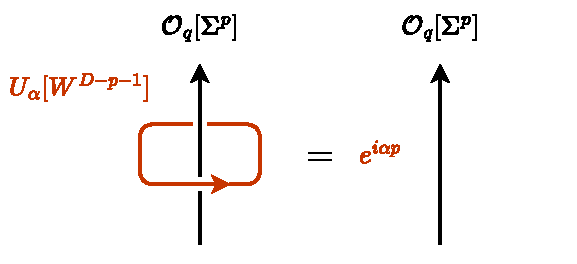
\includegraphics{figures/one-form_act.pdf}

}

}

\end{minipage}%
%
\begin{minipage}[t]{0.50\linewidth}

{\centering 

\raisebox{-\height}{

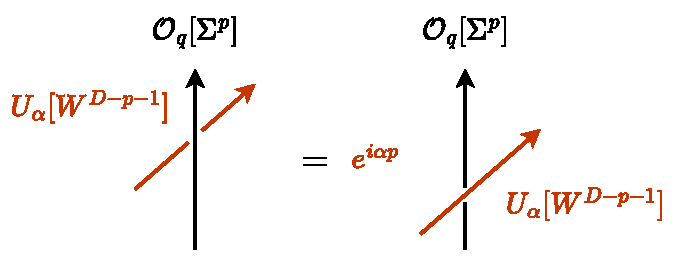
\includegraphics{figures/one_form_passing.pdf}

}

}

\end{minipage}%

\caption{\label{fig-one-form}Action of \(p\)-form symmetry operator
\(U_\alpha[W^{D-p-1}]\) on a \(p\)-dimensional operator
\(\mathcal{O}_q[\Sigma^p]\) of \(p\)-form charge \(q\).}

\end{figure}

\bookmarksetup{startatroot}

\hypertarget{sec-vector}{%
\chapter{Vector}\label{sec-vector}}

\bookmarksetup{startatroot}

\hypertarget{references}{%
\chapter*{References}\label{references}}
\addcontentsline{toc}{chapter}{References}

\markboth{References}{References}

\printbibliography[heading=none]




\end{document}
